\chapter{Browser Cache Analyzer}

\textit{Browser Cache Analyzer} è l'applicazione che è stata sviluppata per eseguire l'analisi della memoria cache dei browser presi in esame.

Permette di ottenere un'anteprima del contenuto lasciando decidere all'utente se effettuarne una successiva estrazione, creando una copia dei dati presenti in memoria cache e fornendo un report finale in formato Html per consentire una più facile consultazione dei risultati.

Progettata per sistemi Windows, presenta un'architettura divisa in \textit{moduli}. Questo la rende flessibile, permettendo di aggiungere nuove funzionalità, come ad esempio il supporto ad altri browser.

\subsection{Implementazione: linguaggi e librerie utilizzate}
Il corpo principale dell'applicazione è stato scritto con il linguaggio di programmazione \textbf{\textit{Python}} mentre la creazione e la gestione dell'interfaccia grafica è affidata al framework \textbf{\textit{Qt}}. Ci si è avvalso anche dell'utilizzo di librerie di terze parti come \textbf{\textit{Psutil}} per informazioni sui processi in uso dal sistema operativo o del programma \textbf{\textit{PyInstaller}} per la creazione del file eseguibile.

\clearpage
\subsubsection{Python}
\nocite{Python}
Alla fine degli anni 80, l'olandese Guido van Rossum iniziò a sviluppare un linguaggio di programmazione che facesse della semplicità uno dei suoi maggiori punti di forza: il \textbf{\textit{Pyhton}}. 

Python è un linguaggio multi-piattaforma ed orientato agli oggetti che supporta caratteristiche quali il \textit{dynamic typing}, che evita errori di tipo sui valori delle varie operazioni, o la \textit{name resolution}, che determina a quale identificatore riferirsi in uno specifico contesto, permettendo così di associare lo stesso nome anche ad oggetti differenti durante l'esecuzione del programma. I blocchi di istruzione all'interno dell'applicazione vengono delimitati dall'intentazione e non da parentesi, garantendo così un'alta leggibilità del codice. Pyhton prevede che la gestione della memoria sia a carico di un \textit{garbage-collector}.

Come tutti i linguaggi interpretati, le sue prestazioni non possono essere comparate a quelle dei linguaggi compilati, specie per applicazioni che richiedono un elevato carico computazionale, ma risultano in linea o superiori a quelle degli altri linguaggi interpretati.

Anche grazie alla sua filosofia, cioè quella di un linguaggio che presenta un elevato numero di librerie standard e al contempo di essere altamente estensibile, è possibile introdurre tutti i moduli per le funzionalità richieste. 
\'E anche possibile scrivere ed integrare estensioni C / C++, potendo così sfruttare le elevate prestazioni di un linguaggio compilato ove richiesto, continuando a beneficiare nel contempo della versatilità del Python.  

\subsubsection{Qt e PyQt} 
\nocite{Qt}
\nocite{PyQt}
Lo sviluppo di \textbf{\textit{Qt}} è iniziato nel 1990 da parte di Eirik Chambe-Eng and Haavard Nord della compagnia norvegese Trolltech. Qt è un framework multi-piattaforma per lo sviluppo di applicazioni in ambiente desktop, embedded e mobile. Scritto in C++, grazie al preprocessore \textit{MOC} (Meta-Object Compiler) ne estende le funzionalità.
Prima della compilazione, il MOC effettua un parsing del codice sorgente in Qt-extended C++ generando un codice conforme al C++. 

Fra le caratteristiche aggiunte, la principale è quella riguardante i \textit{segnali e slot}, utilizzati per la comunicazione fra i vari oggetti dell'applicazione. 

\begin{figure}[htpb]
	\begin{center}
		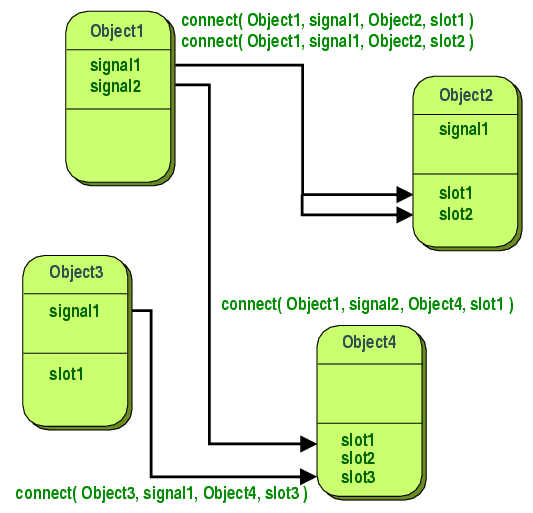
\includegraphics[scale=0.5]{Signal_slot_view.png}
	\end{center}
	\caption[Segnali e slot]{Segnali e slot \footnotemark}
\end{figure}
\footnotetext{\url{http://doc.qt.io/qt-5/signalsandslots.html}}


Al verificarsi di un evento, ad esempio la pressione di un tasto, viene emesso un segnale. Il segnale viene intercettato da uno slot, cioè una funzione con il compito di gestirlo. 
Segnali e slot sono collegati in maniera \textit{loosely coupled}, cioè la classe che emette il segnale non ha conoscenza dello slot che andrà a ricevere il segnale. Sarà il meccanismo Qt che si occupa di gestire i segnali e gli slot a far si che il giusto slot venga richiamato, con i giusti parametri, alla ricezione del segnale. I segnali sono \textit{type safe}, ovvero la signature di un segnale deve combaciare con quella dello slot ricevente. Un segnale è una funzione pubblica e può essere emesso ovunque all'interno dell'applicazione, anche se vi è la raccomandazione di emetterlo dalla classe che lo ha generato o dalle sue sottoclassi.

Così come le classi che emettono il segnale, anche le funzioni che li ricevono non hanno conoscenza dei segnali ai quali sono collegate. Possono essere usate sia per connettere segnali provenienti dai vari oggetti oppure essere utilizzate come normali funzioni, garantendo in questo modo che i componenti siano tra loro indipendenti. Lo slot viene eseguito immediatamente alla ricezione del segnale in modo totalmente indipendente dall'esecuzione della GUI mentre il codice successivo all'istruzione \textit{emit} nella classe che ha emesso il segnale, sarà eseguito non appena lo slot avrà eseguito il \textit{return} tranne in caso di \textit{queued connections} in cui sarà lo slot ad essere eseguito successivamente al codice seguente l'istruzione \textit{emit}.

I segnali, che non possono effettuare il return essendo di tipo \textit{void}, vengono generati dal MOC e non vengono implementati nel file sorgente. 

Per poter utilizzare il framework Qt con Python è stato necessario utilizzare \textbf{\textit{PyQt}}. PyQt permette di effettuare un \textit{binding}, cioè un collegamento, tra il Python e il framework Qt. Questi collegamenti sono implementati tramite moduli Python contenenti più di 1000 classi.

Sviluppato dalla \textit{Riverbank}, il framework PyQt include astrazioni per una moltitudine di oggetti quali il meccanismo per la gestione degli slot e dei segnali, network sockets, threads, Unicode, regular expressions, SQL databases, SVG, OpenGL ed altri ancora. Possiede
anche un web browser pienamente funzionante ed un insieme di GUI widgets.

Un altro componente importante presente in PyQt è il \textbf{\textit{Qt Designer}}, strumento che permette la creazione di interfacce grafiche. 
Le interfacce vengono create disponendo gli oggetti su quella che diventerà una finestra dell'applicazione, facilitando la disposizione degli stessi in layout, permettendo di settarne le proprietà e consentendo anche la creazione delle connessioni fra segnali e slot dei vari oggetti.

\clearpage

\begin{figure}[htpb]
	\begin{center}
		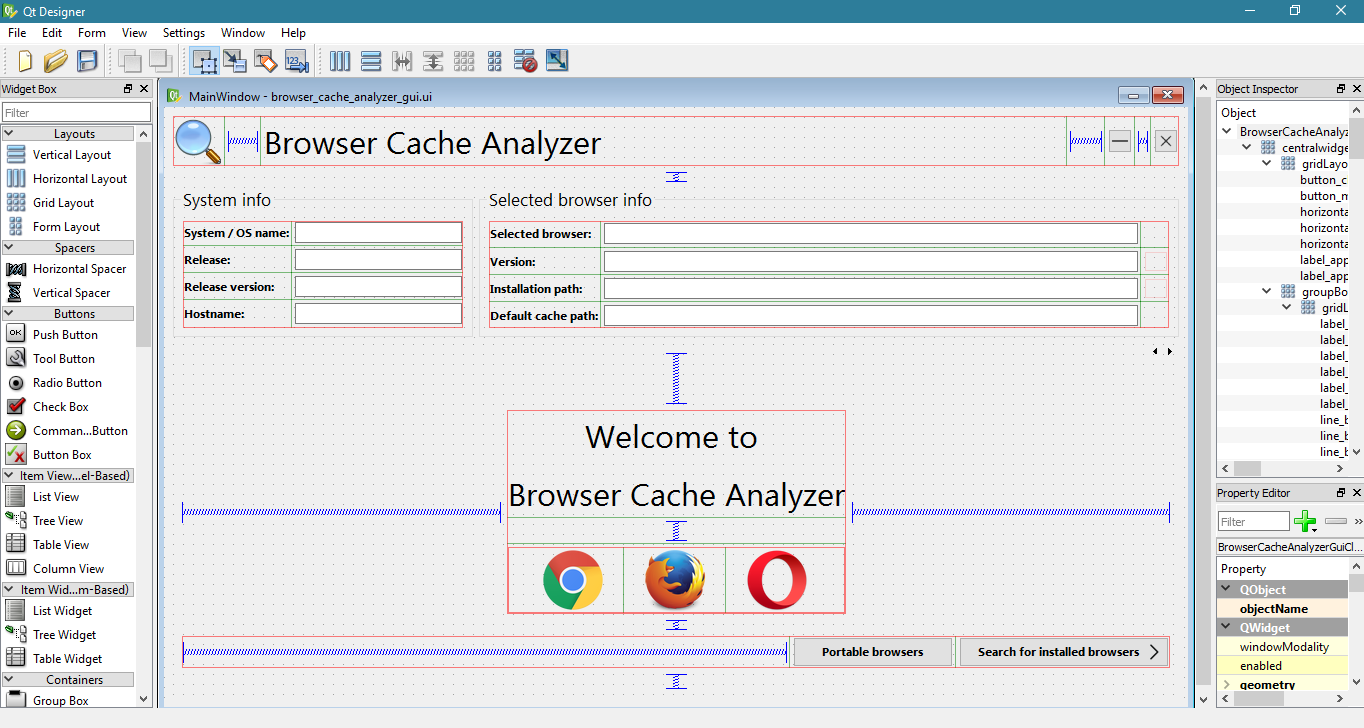
\includegraphics[scale=0.42]{Welcome_screen_designer.png}
	\end{center}
	\caption[Schermata di benvenuto dell'applicazione in QtDesigner]{Schermata di benvenuto dell'applicazione in QtDesigner}
\end{figure}

PyQt inoltre presenta anche un insieme di \textit{utilities} quali:

\begin{itemize}
	\item{pyuic4: corrisponde all'utility \textit{uic} di Qt. Converte le GUI create con QtDesigner in codice Python}
	\item{pyrcc4: corrisponde all'utility \textit{rcc} di Qt. Incorpora risorse esterne (ad esempio icone ed immagini) descritte in un file all'interno di un modulo Python }
\end{itemize} 

\clearpage

\subsubsection{Psutil}
\textbf{\textit{Psutil}} \footnote{\url{https://pypi.python.org/pypi/psutil}} è una libreria multi-piattaforma per Python. Fornisce \textit{utilities} per ottenere informazioni sui processi in esecuzione nel sistema ed utilizzo delle varie risorse (memoria, disco, rete). Implementa anche funzionalità e comandi offerti dalla \textit{command line} come ps, top, lsof, netstat, ifconfig, who, df, kill, free ed altre.

\subsubsection{PyInstaller}
\textbf{\textit{PyInstaller}} \footnote{\url{http://www.pyinstaller.org/}} è un programma che permette la creazione di eseguibili \textit{stand alone} a partire da sorgenti Python. Multi-piattaforma, utilizza il supporto del supporto del sistema operativo per il caricamento di librerie dinamiche, assicurando così piena compatibilità con \textit{packages} di terze parti come PyQt.
\clearpage

\subsection{Descrizione delle componenti}
Di seguito viene fornita una visione della struttura completa dell'applicazione e ne verranno illustrati i vari moduli che la compongono.

\begin{figure}[htpb]
	\begin{center}
		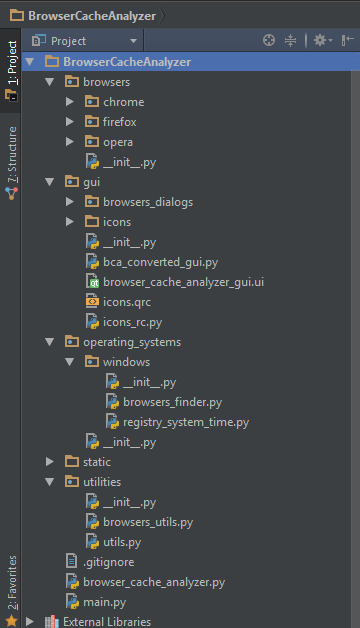
\includegraphics[scale=0.8]{Struttura_applicazione.png}
	\end{center}
	\caption[Struttura dell'applicazione Browser Cache Analyzer]{Struttura dell'applicazione Browser Cache Analyzer}
\end{figure}

\subsubsection{Modulo Browser}
Il modulo \textbf{\textit{Browsers}} è il modulo contenente la logica e le funzioni che permettono di eseguire l'analisi e l'esportazione del contenuto della memoria cache. 
Al suo interno sono contenuti altri moduli, uno per ogni browser preso in esame. 
La scelta di creare il modulo \textit{browsers} è stata presa per poter separare la logica di funzionamento dell'applicazione da quella dei browser. In questo modo aggiungere un nuovo browser o modificare il comportamento di uno già presente, ad esempio a seguito di modifiche o nuove implementazioni della memoria cache da parte del produttore, comporta solo minime modifiche al codice dell'applicazione, volte solo all'aggiunta delle nuove funzionalità.

\begin{figure}[htpb]
	\begin{center}
		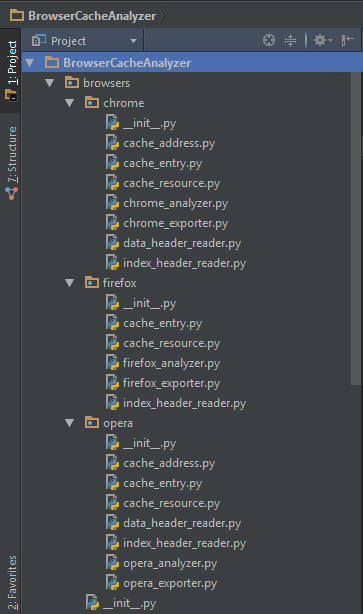
\includegraphics[scale=0.6]{Modulo_browsers.png}
	\end{center}
	\caption[Browser Cache Analyzer: modulo \textbf{\textit{browsers}}]{Browser Cache Analyzer: modulo \textbf{\textit{browsers}}}
\end{figure}

%Si possono osservare i vari file che al loro interno presentano classi e funzioni che ricalcano gli oggetti presenti in memoria cache. Ad %esempio le funzioni \textit{read_index_header}  

